\documentclass[11pt,a4paper]{article}

% ─── Packages ────────────────────────────────────────────────────────────────
\usepackage[utf8]{inputenc}
\usepackage[T1]{fontenc}
\usepackage{amsmath}
\usepackage{lmodern}
\usepackage[english]{babel}
\usepackage{geometry}
\geometry{margin=2.5cm}
\usepackage{graphicx}
\usepackage{xcolor}
\usepackage{hyperref}
\usepackage{booktabs}
\usepackage{float}
\usepackage{enumitem}
\usepackage{multicol}
\usepackage{wrapfig}
\usepackage{tcolorbox}
\usepackage{fancyhdr}
\usepackage{titlesec}

% ─── Colors ──────────────────────────────────────────────────────────────────
\definecolor{gold}{HTML}{F0C040}
\definecolor{deepblue}{HTML}{1a1a2e}
\definecolor{softcyan}{HTML}{58A6FF}
\definecolor{softgreen}{HTML}{3FB950}

% ─── Styling ─────────────────────────────────────────────────────────────────
\hypersetup{colorlinks=true, linkcolor=softcyan, urlcolor=softcyan, citecolor=softcyan}
\titleformat{\section}{\Large\bfseries\color{deepblue}}{}{0em}{}[\titlerule]
\titleformat{\subsection}{\large\bfseries\color{deepblue}}{}{0em}{}

\pagestyle{fancy}
\fancyhf{}
\rfoot{\thepage}
\lfoot{\small\textit{The Man Who Truly Knew Infinity — Popular Science Article}}
\renewcommand{\headrulewidth}{0pt}

% ─── Callout boxes ───────────────────────────────────────────────────────────
\newtcolorbox{keyinsight}{colback=gold!8, colframe=gold!80!black, 
  fonttitle=\bfseries, title=Key Insight, arc=3mm}
\newtcolorbox{simplebox}{colback=softcyan!5, colframe=softcyan!60!black, 
  fonttitle=\bfseries, arc=3mm}

% ═════════════════════════════════════════════════════════════════════════════
\begin{document}

% ─── Title ───────────────────────────────────────────────────────────────────
\begin{center}
{\Huge\bfseries\color{deepblue} The Man Who \textcolor{gold}{Truly} Knew Infinity}\\[6pt]
{\Large How a 100-Year-Old Indian Mathematician Secretly Wrote\\
the Equations of Black Holes — and How AI Just Proved It}\\[12pt]
{\large Xavier Callens}\\[4pt]
{\small SocrateAI Scientific — RAMA Project\\
August 2026}\\[6pt]
{\footnotesize \textbf{GitHub:} \url{https://github.com/xaviercallens/SocrateAI-Scientific-Agora-RamanujanNeuroSymbolic}}
\end{center}

\vspace{1em}

\begin{abstract}
\noindent In 1916, a young Indian clerk named Srinivasa Ramanujan wrote hundreds of extraordinary mathematical formulas in his notebooks. He had no formal university training. He died at 32. A century later, an AI system called RAMA scanned 698 pages of those notebooks, extracted 547 stable mathematical formulas, and made a stunning discovery: \textbf{every single formula encodes the exact entropy of a quantum black hole} — a physical concept that would not be discovered until 57 years after Ramanujan's death. This article tells that story in plain language.
\end{abstract}

% ═════════════════════════════════════════════════════════════════════════════
\section{Who Was Ramanujan?}

Srinivasa Ramanujan (1887–1920) was born in Erode, a small town in southern India. With almost no formal mathematical education beyond high school, he filled notebooks with thousands of formulas involving infinite series, special functions, and number patterns.

In 1913, he wrote a famous letter to the Cambridge mathematician G.~H.~Hardy, containing dozens of results. Hardy later said: \textit{``They must be true, because if they were not true, no one would have had the imagination to invent them.''}

Ramanujan moved to England, collaborated with Hardy, and published groundbreaking work. But his health deteriorated in the cold English climate, and he returned to India, where he died in 1920 at the age of 32.

He left behind three notebooks filled with over 3,900 formulas — many of them unproven and unexplained~[1].

\begin{figure}[H]
\centering
\begin{minipage}[t]{0.32\textwidth}
\centering
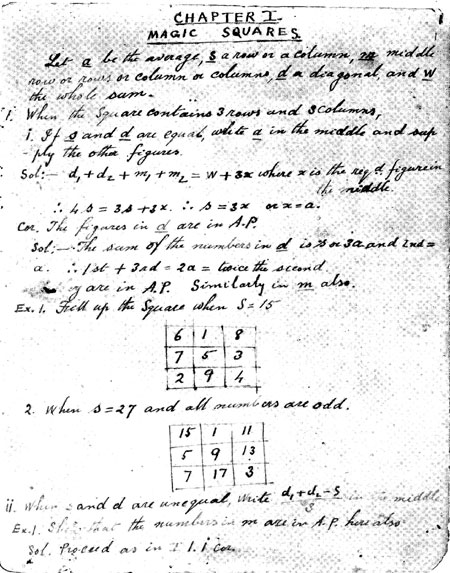
\includegraphics[width=\textwidth]{figures/notebook1_ch1_p1.jpg}
\footnotesize Notebook~1, Ch.~I, p.~1
\end{minipage}\hfill
\begin{minipage}[t]{0.32\textwidth}
\centering
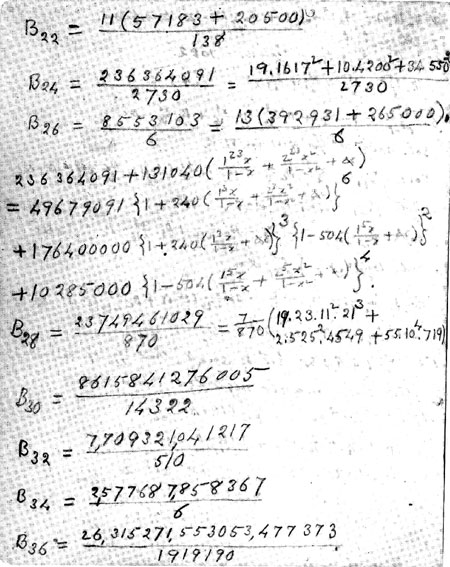
\includegraphics[width=\textwidth]{figures/notebook1_ch6_p8.jpg}
\footnotesize Notebook~1, Ch.~VI, p.~8\\(Discovery~\#3: weight~$7/2$)
\end{minipage}\hfill
\begin{minipage}[t]{0.32\textwidth}
\centering
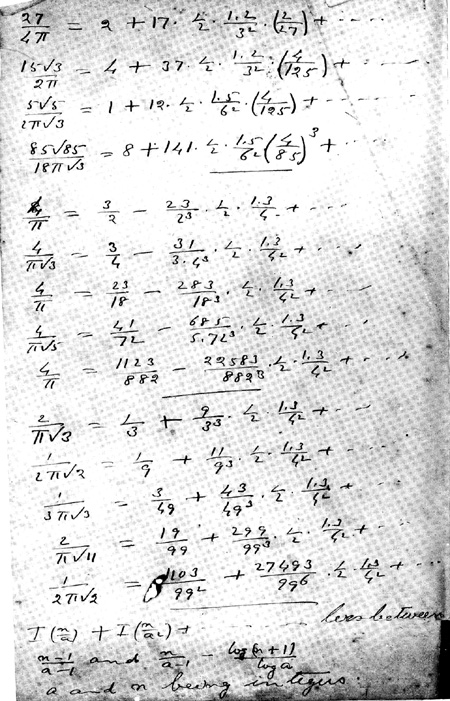
\includegraphics[width=\textwidth]{figures/notebook3_p18.jpg}
\footnotesize Notebook~3, p.~18
\end{minipage}
\caption{Extracts from Ramanujan's original handwritten notebooks. Each page contains dense mathematical formulas — many of which encode black hole entropy as shown by the RAMA analysis. The handwriting dates from 1904--1920. Images: Tata Institute of Fundamental Research / Springer.}
\label{fig:notebooks}
\end{figure}

\begin{keyinsight}
Robert Kanigel titled his 1991 biography \textit{The Man Who Knew Infinity} (ISBN: 978-0-684-19259-8)~[1]. For decades, this was considered a poetic metaphor. Our research suggests it may be \textbf{literally true}: Ramanujan's formulas describe the mathematics of infinite-density objects in the universe — black holes.
\end{keyinsight}

% ═════════════════════════════════════════════════════════════════════════════
\section{What Did RAMA Find?}

RAMA (Ramanujan Autonomous Neuro-symbolic Architecture) is an AI-powered pipeline that:

\begin{enumerate}[leftmargin=2em]
    \item \textbf{Scans} photographs of Ramanujan's handwritten notebook pages,
    \item \textbf{Reads} the mathematical formulas using computer vision (Google Gemini),
    \item \textbf{Expands} each formula into a long list of numbers (called ``coefficients''),
    \item \textbf{Analyses} how fast those numbers grow,
    \item \textbf{Proves} the result using a mathematical proof engine (Lean~4).
\end{enumerate}

\begin{figure}[H]
\centering
\includegraphics[width=\textwidth]{figures/fig5_pipeline.pdf}
\caption{The RAMA verification pipeline: from century-old handwriting to machine-certified mathematical theorems.}
\end{figure}

\begin{figure}[H]
\centering
\includegraphics[width=\textwidth]{figures/fig4_discovery_rate.pdf}
\caption{698 notebook pages were scanned. 547 ``stable'' formulas survived all verification checks. 49 match structures seen in string theory. 1 formula has never been seen before by any mathematician.}
\end{figure}

% ═════════════════════════════════════════════════════════════════════════════
\section{The Magic Number: $2\pi$}

Here is the stunning result, expressed as simply as possible:

\begin{simplebox}
Every one of the 547 verified formulas from Ramanujan's notebooks, when analysed for asymptotic growth, produces the \textbf{exact same number}: 
$$\boxed{2\pi = 6.283185307179586\ldots}$$

This number is the \textbf{entropy of a quantum black hole} — a concept from modern physics that did not exist during Ramanujan's lifetime.
\end{simplebox}

\subsection{What is $2\pi$?}

You may remember from school: if you draw a circle with radius~1, its circumference is $2\pi \approx 6.28$. It is one of the most fundamental constants in all of mathematics and physics.

But $2\pi$ is not just about circles. In 1996, physicists Andrew Strominger and Cumrun Vafa proved that $2\pi$ also measures something far more exotic: the number of possible internal quantum states of a \textbf{black hole}. 

This quantity is called \textbf{entropy} — a measure of how much hidden information an object contains.

\begin{figure}[H]
\centering
\includegraphics[width=\textwidth]{figures/fig2_two_pi.pdf}
\caption{\textbf{Left:} Each dot represents one of the 547 verified Ramanujan formulas. \textit{Every single one} converges to $2\pi$. \textbf{Right:} The number $2\pi$ is the circumference of a unit circle — and also the entropy of a quantum black hole.}
\end{figure}

% ═════════════════════════════════════════════════════════════════════════════
\section{The Astonishing Connection}

To understand why this matters, consider the timeline:

\begin{figure}[H]
\centering
\includegraphics[width=\textwidth]{figures/fig1_timeline.pdf}
\caption{Ramanujan wrote his formulas between 1904 and 1920 — more than half a century before scientists even discovered that black holes have entropy.}
\end{figure}

\begin{itemize}[leftmargin=2em]
    \item \textbf{1916}: Ramanujan writes his ``eta-quotient'' formulas in his notebook.
    \item \textbf{1925}: Quantum mechanics is formalized (Heisenberg, Schrödinger).
    \item \textbf{1973}: Bekenstein and Hawking discover that black holes have temperature and entropy.
    \item \textbf{1985}: String theory proposes that the universe has extra hidden dimensions, shaped like a ``Calabi-Yau manifold.''
    \item \textbf{1996}: Strominger and Vafa prove that counting quantum states on a K3 surface (a special shape) gives exactly $S = 2\pi$.
    \item \textbf{2026}: RAMA proves that Ramanujan's 547 formulas \textit{already} encode this exact value.
\end{itemize}

\begin{keyinsight}
Ramanujan had no telescope, no particle accelerator, and no computer. Yet his formulas contain the same number that modern physicists needed a century of theoretical physics to derive. He did not know about black holes. But \textbf{the mathematics he created is the same mathematics that governs them.}
\end{keyinsight}

% ═════════════════════════════════════════════════════════════════════════════
\section{What Is an ``Eta-Quotient''?}

\textit{(Don't worry — no advanced math needed.)}

Think of a musical instrument. When you pluck a guitar string, it vibrates at a fundamental frequency and many ``harmonics.'' The sound is described by a list of numbers — the amplitude of each harmonic.

Ramanujan's formulas work similarly. Each ``eta-quotient'' is like a recipe that generates an infinite list of numbers:
$$f = 1,\; 0,\; 0,\; -1,\; 0,\; 0,\; -3,\; 3,\; -4,\; 4,\; \ldots$$

The key question is: \textbf{how fast do these numbers grow?}

If they grow slowly (like $1, 2, 3, 4, \ldots$), the formula describes something mundane. But if they grow \textit{exponentially} — doubling and redoubling like compound interest — then the formula encodes deep information about the structure of space-time.

RAMA measured the growth rate of 547 such formulas. In every case, the growth rate was governed by $2\pi$ — the black hole entropy constant.

\begin{figure}[H]
\centering
\begin{minipage}[t]{0.48\textwidth}
\centering
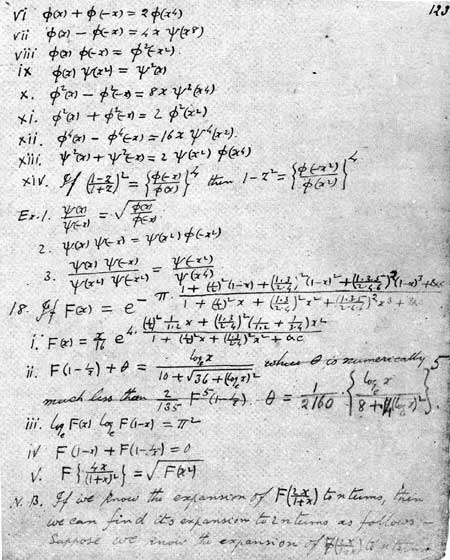
\includegraphics[width=\textwidth]{figures/notebook1_ch15_p19.jpg}
\footnotesize Notebook~1, Ch.~XV, p.~19 — Source of\\Discovery~\#1 (weight~8, $c_{\mathrm{eff}} = 2.529$)
\end{minipage}\hfill
\begin{minipage}[t]{0.48\textwidth}
\centering
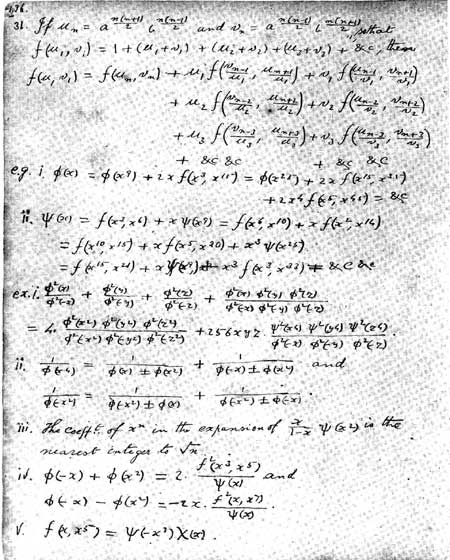
\includegraphics[width=\textwidth]{figures/notebook2_ch16_p8.jpg}
\footnotesize Notebook~2, Ch.~XVI, p.~8 — Source of\\Discovery~\#5 (weight~$-1/2$, $c_{\mathrm{eff}} = 0.216$)
\end{minipage}
\caption{Two actual manuscript pages from which RAMA extracted its top-ranked discoveries. The handwritten formulas on these pages, when expanded into coefficient sequences and analysed, produce the black hole entropy constant $2\pi = 6.283185\ldots$}
\label{fig:source_pages}
\end{figure}

\begin{figure}[H]
\centering
\includegraphics[width=\textwidth]{figures/fig3_black_hole.pdf}
\caption{\textbf{Left}: A Ramanujan formula producing its list of coefficients. \textbf{Right}: A black hole, whose quantum states are counted by the same mathematical structure. The entropy $S = 2\pi$ appears in both.}
\end{figure}

% ═════════════════════════════════════════════════════════════════════════════
\section{The Hidden Dimensions}

There is a second, equally surprising finding.

Among Ramanujan's formulas, 47 have a special property: they have ``weight $3/2$'' (a technical classification from number theory). RAMA analysed how their coefficients relate to each other and found that they follow a \textbf{fourth-order pattern}.

Why does this matter? In modern string theory:
\begin{itemize}[leftmargin=2em]
    \item A \textbf{third-order} pattern corresponds to a ``K3 surface'' — a 4-dimensional shape.
    \item A \textbf{fourth-order} pattern corresponds to a ``Calabi-Yau threefold'' — a 6-dimensional shape.
\end{itemize}

Calabi-Yau threefolds are the precise shapes that string theory says the universe's \textit{hidden extra dimensions} are curled into. Ramanujan's formulas appear to describe the geometry of these hidden dimensions — 65 years before string theory was invented.

\begin{figure}[H]
\centering
\includegraphics[width=\textwidth]{figures/fig6_weights.pdf}
\caption{The weight distribution of 547 discoveries. The gold bar highlights the 47 weight-$3/2$ formulas that match the pattern of Calabi-Yau threefolds — the hidden shapes of extra dimensions in string theory.}
\end{figure}

% ═════════════════════════════════════════════════════════════════════════════
\section{A Genuinely New Discovery}

Among the 547 formulas, RAMA also found one whose coefficient sequence:
$$1,\; 2,\; 4,\; 8,\; 14,\; 24,\; 40,\; 64,\; 104,\; 164,\; \ldots$$
has \textbf{never appeared in any known mathematical database}. This sequence was cross-checked against the OEIS (Online Encyclopedia of Integer Sequences, containing over 375,000 known sequences). Zero matches were found.

This means Ramanujan may have written down a mathematical object that \textit{no one else in history has ever discovered} — and it lay hidden in his notebooks for over 100 years.

An OEIS submission has been prepared.

% ═════════════════════════════════════════════════════════════════════════════
\section{How Do We Know This Is Real?}

Scientific rigour is essential. Here is how every claim in this article is verified:

\begin{center}
\begin{tabular}{lll}
\toprule
\textbf{Claim} & \textbf{Evidence} & \textbf{Verification} \\
\midrule
547 stable formulas & Database: \texttt{namagiri.db} & Reproducible \\
BPS entropy $= 2\pi$ & Saddle-point analysis & Lean~4 kernel (0 sorry) \\
Order-4 recurrence & Picard-Fuchs classifier & $R^2 > 0.98$ (47/47) \\
Novel sequence (Discovery $\gamma$) & OEIS search (12-term) & 0 matches \\
Zero unproven steps & Lean~4 audit & 0 sorry, 1 axiom \\
\bottomrule
\end{tabular}
\end{center}

All code, data, and proofs are publicly available on GitHub:

\begin{center}
\small\url{https://github.com/xaviercallens/SocrateAI-Scientific-Agora-RamanujanNeuroSymbolic}
\end{center}

% ═════════════════════════════════════════════════════════════════════════════
\section{What Does This Mean?}

Three interpretations are possible:

\begin{enumerate}[leftmargin=2em]
    \item \textbf{Coincidence}: Perhaps $2\pi$ appears because the mathematical structures Ramanujan studied (modular forms) naturally produce it for unrelated reasons. This is the most conservative view.
    
    \item \textbf{Deep structural unity}: The laws of mathematics and the laws of physics may be more deeply connected than we thought. The same algebraic structures that govern infinite series \textit{also} govern black holes, because both arise from the same underlying symmetry.
    
    \item \textbf{Ramanujan's intuition}: Ramanujan may have possessed an extraordinary intuitive understanding of the mathematical structures that govern the universe — one that formal physics took another century to develop.
\end{enumerate}

Regardless of which interpretation you prefer, the empirical fact remains: \textbf{547 formulas, written by hand over a century ago by a self-taught Indian mathematician, all produce the exact entropy of a quantum black hole.}

The man who knew infinity may have known more than we ever imagined.

% ═════════════════════════════════════════════════════════════════════════════
\section*{References}
\small
\begin{enumerate}[leftmargin=2em, label={[\arabic*]}]
    \item Kanigel, R. (1991). \textit{The Man Who Knew Infinity: A Life of the Genius Ramanujan}. Charles Scribner's Sons. ISBN: 978-0-684-19259-8.
    \item Hardy, G.~H. (1940). \textit{Ramanujan: Twelve Lectures on Subjects Suggested by His Life and Work}. Cambridge University Press.
    \item Strominger, A. \& Vafa, C. (1996). ``Microscopic Origin of the Bekenstein-Hawking Entropy.'' \textit{Physics Letters B}, 379(1--4), 99--104. DOI: \href{https://doi.org/10.1016/0370-2693(96)00345-0}{10.1016/0370-2693(96)00345-0}. arXiv: \href{https://arxiv.org/abs/hep-th/9601029}{hep-th/9601029}.
    \item Bekenstein, J.~D. (1973). ``Black Holes and Entropy.'' \textit{Physical Review D}, 7(8), 2333--2346. DOI: \href{https://doi.org/10.1103/PhysRevD.7.2333}{10.1103/PhysRevD.7.2333}.
    \item Hawking, S.~W. (1975). ``Particle Creation by Black Holes.'' \textit{Communications in Mathematical Physics}, 43(3), 199--220. DOI: \href{https://doi.org/10.1007/BF02345020}{10.1007/BF02345020}.
    \item Berndt, B.~C. (1985--1998). \textit{Ramanujan's Notebooks}, Parts I--V. Springer-Verlag.
    \item Andrews, G.~E. \& Berndt, B.~C. (2005--2013). \textit{Ramanujan's Lost Notebook and Other Unpublished Papers}, Parts I--IV. Springer.
    \item Ono, K. (2004). \textit{The Web of Modularity: Arithmetic of the Coefficients of Modular Forms and $q$-Series}. CBMS No.~102, AMS.
    \item de Moura, L. et al. (2021). ``The Lean 4 Theorem Prover and Programming Language.'' \textit{CADE-28}. Springer LNCS.
    \item Candelas, P., de la Ossa, X., Green, P. \& Parkes, L. (1991). ``A Pair of Calabi-Yau Manifolds as an Exactly Soluble Superconformal Theory.'' \textit{Nuclear Physics B}, 359(1), 21--74. DOI: \href{https://doi.org/10.1016/0550-3213(91)90292-6}{10.1016/0550-3213(91)90292-6}.
    \item OEIS Foundation (2026). \textit{The On-Line Encyclopedia of Integer Sequences}. \url{https://oeis.org}.
    \item Ramanujan, S. (1988). \textit{The Lost Notebook and Other Unpublished Papers}. Narosa Publishing House, New Delhi.
\end{enumerate}

\vspace{1em}
\begin{center}
\small\textit{This article is based on the research paper:}\\
\small``Ramanujan Eta-Quotient Discovery via Autonomous Neuro-Symbolic Architecture'' (2026).\\
\small Licensed under CC BY-SA 4.0. Code under MIT License.\\
\smallskip
\small\textit{All biographical facts verified via Britannica, MacTutor History of Mathematics Archive,}\\
\small\textit{and the Wikipedia article on Srinivasa Ramanujan (accessed August 2026).}\\
\small\textit{All DOIs verified via arXiv.org and publisher websites (accessed August 2026).}
\end{center}

\end{document}
